\documentclass{article}

\usepackage{PRIMEarxiv}

\usepackage[utf8]{inputenc} % allow utf-8 input
\usepackage[T1]{fontenc}    % use 8-bit T1 fonts
\usepackage{hyperref}       % hyperlinks
\usepackage{url}            % simple URL typesetting
\usepackage{booktabs}       % professional-quality tables
\usepackage{amsfonts}       % blackboard math symbols
\usepackage{amsmath}
\usepackage{amssymb}
\usepackage{amsthm}
\usepackage{nicefrac}       % compact symbols for 1/2, etc.
\usepackage{microtype}      % microtypography
\usepackage{graphicx}
\usepackage{adjustbox}
\usepackage[section]{placeins}
\usepackage[dvipsnames]{xcolor}
\graphicspath{{media/}}     % figures live under media/

\hypersetup{colorlinks=true, linkcolor=blue!50!black, citecolor=blue!50!black, urlcolor=blue!50!black}

\theoremstyle{plain}
\newtheorem{proposition}{Proposition}
\theoremstyle{definition}
\newtheorem{definition}{Definition}

% Notation used throughout
\newcommand{\WR}{\mathrm{WR}}
\newcommand{\JA}{J_A}
\newcommand{\JB}{J_B}
\newcommand{\SR}{\mathrm{SR}_\Delta}
\newcommand{\Qmax}{Q_{\max}}
\newcommand{\Muni}{M_{\mathrm{uni}}}
\newcommand{\vmax}{v_{\max}}

% Running head: short title instead of the template placeholder
\fancyhf{}
\rhead{\textit{Fairness, efficiency, and strategic behaviour in shared GPU allocation}}
\cfoot{\thepage}

%% Title
\title{Fairness, Efficiency, and Strategic Behaviour in Shared GPU Allocation
\thanks{\textit{\underline{Note}}: Course project report, Foundations of Artificial Intelligence. 
Code, data and figures: \url{https://github.com/kalpshah18/Shared-GPU-Allocation}.}
}

\author{
  Aayush Kuloor, Harsh Dhru, Raj Modi, Kalp Shah \\
  Indian Institute of Technology Gandhinagar \\
  Gandhinagar, India \\
  \texttt{\{aayush.kuloor, harsh.dhru, raj.modi, kalp.shah\}@iitgn.ac.in} \\
}

\begin{document}
\maketitle

\begin{abstract}
Shared GPU clusters divide scarce accelerators among users who know the value of their own jobs and may misreport it.
We study a repeated, unit-demand allocation model in which $n$ users compete for $k$ identical GPUs in each of $T$ rounds.
Five baseline mechanisms are compared on welfare, long-run fairness, waiting time and the gain from bounded misreporting: random allocation, round-robin, greedy allocation by reported value, a history-penalised score, and a $k$-unit Vickrey auction.
All comparisons use paired valuation traces, 30 locked seeds and bootstrap intervals, and the simulator is validated by exhaustive tests on small instances.
Value-aware rules reach first-best welfare under truthful reports but concentrate service when users differ or demand persists.
A history penalty recovers most of the fairness at a welfare cost below one percent, but the penalty needed to deter a lie grows as the lie gets milder, and a planning attacker with a 40-round horizon profits against the score rule even at penalty $\lambda=2$.
We therefore propose two non-monetary mechanisms, Karma-Cap and Rank-Cap, that add a provable waiting bound, and we evaluate them with component ablations, adaptive policy choice, an offline welfare benchmark that enforces the same service requirement, and diagnostics of their failure modes.
The waiting bound costs about 5 percent of welfare on homogeneous demand and brings the welfare ratio down to between 0.72 and 0.81 under heterogeneous demand and under persistent demand with a preserved value distribution.
Neither mechanism is strategyproof: the deterrence of Karma-Cap reverses when all other users inflate, and Rank-Cap is profitably attacked by a planner that updates its report history.
The evidence comes from simulation and does not establish dynamic strategyproofness.
\end{abstract}

\keywords{GPU allocation \and fair resource allocation \and mechanism design \and strategic behaviour \and simulation}

\section{Introduction}
\label{sec:intro}

Machine-learning workloads compete for expensive shared accelerators, and the scheduling rule determines both cluster efficiency and how long each user waits.
Production schedulers already handle priorities, heterogeneous accelerators, placement and long-running jobs \cite{gu2019tiresias,narayanan2020gavel}.
Access still matters beyond throughput.
A rule that repeatedly serves the jobs with the largest apparent benefit can starve everyone else, while a rigid equal-time rule wastes compute when job values differ a great deal.

Private information adds a second difficulty.
If allocation depends on a self-reported priority, a user can inflate the report to obtain service, and the scheduler sees only the claim.
A rule that is efficient under truthful reports can therefore perform poorly once users act strategically.
Several GPU schedulers address fairness and incentives in different ways.
Tiresias uses attained service to reduce job completion time, Gavel generalises scheduling policies to heterogeneous accelerators, Themis combines finish-time fairness with a round-by-round auction, and Shockwave uses market-based planning for jobs that adapt during training \cite{gu2019tiresias,narayanan2020gavel,mahajan2020themis,zheng2023shockwave}.

This report studies a narrower question in a stylised model.
The model removes job arrivals, durations, placement and multi-GPU jobs so that scarcity, allocation history and bounded misreporting can be varied one at a time while the information and random inputs are held fixed.
It does not describe a production scheduler and does not claim a new impossibility theorem.

\paragraph{Research question.}
How do simple repeated GPU-allocation mechanisms trade off true social welfare, long-run fairness and empirical resistance to bounded strategic reporting as scarcity, user heterogeneity and temporal demand patterns vary?
The project proposal posed three subsidiary questions.
First, does a moderate history penalty reduce starvation without a large loss of true welfare?
Second, does a stronger penalty change the benefit from strategically timing or inflating reports?
Third, do conclusions based on equal allocation counts survive unequal value distributions or persistent demand?

\paragraph{What this report covers.}
The study has two parts.
The first part implements the evaluation planned in the proposal: five baseline mechanisms, four kinds of reporting policy including a finite-horizon rollout attack, the planned metrics, the experiments E1 to E6 together with the rollout studies E3b and E3c, a sensitivity grid (E7), a timing attack (E8), and an exhaustive validation suite (E0).
Its main findings changed during the work.
An early reading suggested that a history penalty of $\lambda=2$ makes inflation unprofitable, but the penalty that deters a lie grows as the lie gets milder, and a planning attacker still gains at $\lambda=2$.
These findings motivated the second part, which designs two mechanisms with a hard waiting bound (Karma-Cap and Rank-Cap, called M6 and M7), tests them on the same workloads (E9 to E11), and then challenges the results with six further studies on held-out seeds (E12 to E18).

\paragraph{Contributions.}
The report makes the following contributions.
\begin{enumerate}
\item A seeded simulator with a paired-randomness contract, a mechanism interface that covers both payment and non-payment rules, and an exhaustive validation suite with negative controls.
\item A measurement of individual manipulation gain that holds every other user fixed, reported next to the coalition gain, which can have the opposite sign.
\item An evaluation of the five baselines showing that the history penalty needed to deter exaggeration depends on the size of the lie and on the planning ability of the attacker.
\item Two non-monetary mechanisms with a proved waiting bound, and a statement of precisely what they do and do not guarantee, including a proof that rank normalisation is invariant to fixed strictly increasing report distortions.
\item A component study that separates the effect of the waiting cap from the effect of the incentive component, an adaptive-policy game, an exact offline welfare benchmark under the same service constraint, and trace-level diagnostics of how Karma-Cap and Rank-Cap fail.
\end{enumerate}

\paragraph{Organisation.}
Section~\ref{sec:related} reviews related work.
Section~\ref{sec:model} defines the model and metrics, Section~\ref{sec:mechanisms} the mechanisms and their formal properties, and Section~\ref{sec:attackers} the strategic policies.
Section~\ref{sec:protocol} describes the experimental protocol.
Section~\ref{sec:results} reports the results, Section~\ref{sec:discussion} returns to the hypotheses, and Sections~\ref{sec:limits} and~\ref{sec:conclusion} give limitations and conclusions.

\section{Related Work}
\label{sec:related}

\paragraph{GPU cluster scheduling.}
Tiresias prioritises jobs by attained service, using either a discretised Gittins index or a two-dimensional least-attained-service rule \cite{gu2019tiresias}.
The score mechanism studied here has the same shape, because it divides a report by a power of the user's past allocation count.
Gavel expresses scheduling policies as optimisation problems over heterogeneous accelerators and enforces them with a round-based mechanism \cite{narayanan2020gavel}.
Themis introduces finish-time fairness and lets jobs bid for GPUs in auctions run by a central arbiter \cite{mahajan2020themis}.
Shockwave extends market theory to jobs whose throughput changes over time and plans ahead with stochastic dynamic programming \cite{zheng2023shockwave}.
These systems model placement, job structure and heterogeneity that our model omits.
Our model keeps the private-value and repeated-round structure only, which lets us isolate cross-round incentives.

\paragraph{Fair division and dynamic demands.}
Dominant resource fairness generalises max-min fairness to several resource types \cite{ghodsi2011drf}.
Jain's index \cite{jain1984quantitative} and the price of fairness \cite{bertsimas2011price} provide the fairness and efficiency-loss measures we use.
Karma \cite{vuppalapati2023karma} allocates a shared resource under dynamic demands by giving credits to users who donate unused capacity that others borrow, and proves strategy-proofness and fairness properties in that model.
The mechanism we call Karma-Cap is different: it is a uniform-price bid auction in an internal balance with redistribution and a service override, so the published guarantees do not carry over to it.
Fikioris, Agarwal and Tardos show that history-aware dynamic max-min and dominant-resource allocation is not incentive compatible, although it is approximately so \cite{fikioris2021incentives}.
Their result agrees with our finding that a history penalty only partly deters misreporting.
Their demand model is not our private-value unit-demand model.

\paragraph{Repeated mechanism design without money.}
Linking many decisions can discipline reports without transfers \cite{jackson2007linking}, and the idea is also present in storable votes \cite{casella2005storable}.
Artificial currencies convert a one-shot monetary mechanism into a dynamic non-monetary one with vanishing loss \cite{gorokh2021artificial}, and karma economies study stationary equilibria of bidding in a circulating internal currency \cite{elokda2024karma}.
Balseiro, Gurkan and Sun study a principal who repeatedly allocates a single resource among agents with private values and no payments, and who induces truthful reports through promises and threats of future allocations \cite{balseiro2019multiagent}.
M6 borrows the idea that a bid should cost future priority, and M7 borrows the idea that a report is informative mainly relative to the user's own distribution.
We do not claim novelty beyond the combination with a hard waiting bound for unit-demand GPU allocation, and our literature search was not exhaustive.

\paragraph{Bounded-lag scheduling.}
Round-based schedulers in networking, such as deficit round robin \cite{shreedhar1995drr}, serve every active flow in each round, and lottery scheduling allocates shares by randomisation \cite{waldspurger1994lottery}.
The wait cap in M6 and M7 follows the same idea of an explicit service guarantee, without an incentive analysis in these original settings.
The auction baseline follows Vickrey \cite{vickrey1961counterspeculation} and the VCG construction for identical units \cite{nisan2007agt}.

\section{Model and Metrics}
\label{sec:model}

\paragraph{Agents, resources and time.}
There are $n$ unit-demand users and $T$ discrete rounds.
In each round $k<n$ identical GPUs are available and each user can receive at most one.
User $i$ draws a private value $v_{i,t}\in[0,\vmax]$ from a distribution $D_i$ and submits a report $\hat v_{i,t}\in[0,\vmax]$ with $\vmax=1$.
Bounded reports rule out the degenerate case in which an arbitrarily large bid controls the outcome.
A mechanism returns an allocation $x_t\in\{0,1\}^n$ with $\sum_i x_{i,t}=k$ and a payment vector $p_t\ge 0$ with $p_{i,t}=0$ whenever $x_{i,t}=0$.
Payments are zero for the non-payment rules.
Ties are broken by a seeded generator.

\paragraph{History and waiting.}
The public history before round $t$ gives the cumulative allocation $a_i(t)=\sum_{\tau<t}x_{i,\tau}$.
The wait $q_i(t)$ is the number of consecutive rounds before round $t$ in which user $i$ received no GPU, with $q_i(0)=0$.

\paragraph{Utility and welfare.}
User utility is quasi-linear, $u_{i,t}=v_{i,t}x_{i,t}-p_{i,t}$ with $U_i=\sum_t u_{i,t}$, and the gross benefit is $G_i=\sum_t v_{i,t}x_{i,t}$.
Payments are transfers, so social welfare is $W=\sum_i G_i$.
The oracle welfare $W^*$ allocates in every round to the $k$ users with the highest true values, and the welfare ratio is
\begin{equation}
\WR = W/W^*.
\end{equation}

\paragraph{Fairness and waiting metrics.}
With $A_i=a_i(T+1)$, Jain's allocation index is $\JA=(\sum_i A_i)^2/(n\sum_i A_i^2)$.
When the $D_i$ differ, equal service need not mean equal benefit, so we also report $\JB=(\sum_i B_i)^2/(n\sum_i B_i^2)$ with $B_i=G_i/(T\mu_i)$ and $\mu_i=\mathbb{E}_{D_i}[v]$.
Nash social welfare is $\mathrm{NSW}=\sum_i\log(G_i+10^{-8})$.
The maximum wait is $\Qmax=\max_{i,t}q_i(t)$, and with $\Delta=2\lceil n/k\rceil$ (twice the round-robin service cycle) the starvation rate is
\begin{equation}
\SR=\frac{1}{nT}\sum_{i=1}^{n}\sum_{t=1}^{T}\mathbf{1}\{q_i(t)>\Delta\}.
\end{equation}
We also report the 95th percentile of all waiting times.
Price of fairness is $\mathrm{PoF}=(W^*-W_F)/W^*$ for mechanism $F$ under truthful reports.

\paragraph{Manipulation gain.}
Let $\omega$ contain a valuation trace, a tie-breaking stream and a strategic set $S\subseteq[n]$ with $|S|=\lfloor\rho n\rfloor$.
A reporting policy may depend on the current value and the public history.
The proposal defines the manipulation gain of user $i$ as
\begin{equation}
M_i(\sigma_i;\omega)=U_i(\sigma_i,\sigma_{-i};\omega)-U_i(\text{truthful},\sigma_{-i};\omega),
\end{equation}
which changes only user $i$'s policy.
We call the mean of $M_i$ over a set of focal users the unilateral gain $\Muni$, and we also report the fraction of focal users with $M_i>0$.
In each seed, five strategic users are the focal users.
For a focal user in $S$ the comparison is between the run in which all of $S$ deviates and the run in which $S\setminus\{i\}$ deviates.
When $\rho=0$ the focal user is a lone deviator in a truthful population.
The coalition gain compares the run in which all of $S$ deviates with the all-truthful run.
Strategic users crowd each other out, so a negative coalition gain does not imply that an individual is better off truthful.
The price of strategy is $\mathrm{PoS}=(W_{\text{truthful}}-W_{\text{strategic}})/W_{\text{truthful}}$.
Every comparison pairs runs on the same $\omega$.

\paragraph{Incentive terminology.}
A one-round direct mechanism is dominant-strategy incentive compatible (DSIC) when truthful reporting weakly maximises each user's utility for every profile of other reports \cite{nisan2007agt}.
A report-invariant rule is weakly strategyproof because reports cannot affect it.
For history-dependent non-payment rules our experiments measure vulnerability to specified attacks, and simulation cannot establish dynamic strategyproofness.

\section{Mechanisms}
\label{sec:mechanisms}

Table~\ref{tab:mech} lists the mechanisms.
M1 to M5 are the proposal's baselines, and M6 and M7 are the mechanisms designed in this project.

\begin{table}[!htb]
\caption{Mechanisms and their formal properties.}
\label{tab:mech}
\centering
\footnotesize
\setlength{\tabcolsep}{4pt}
\adjustbox{max width=\textwidth}{%
\begin{tabular}{llcccl}
\toprule
ID & Mechanism & Reports & History & Payments & Formal property \\
\midrule
M1 & Random & no & no & no & report-invariant \\
M2 & Round-Robin & no & yes & no & report-invariant; $\Qmax\le\lceil n/k\rceil-1$ \\
M3 & Greedy & yes & no & no & first-best under truthful reports only \\
M4 & Score ($\lambda=1$ by default) & yes & yes & no & $\lambda=0$ gives M3; tested empirically \\
M5 & $k$-unit Vickrey & yes & no & yes & DSIC in each round \\
M6 & Karma-Cap & yes & yes & internal karma & $\Qmax\le W+\lceil n/k\rceil-1$; incentives tested empirically \\
M7 & Rank-Cap & yes & yes & no & same wait bound; invariant to fixed monotone distortions in pure-rank mode \\
\bottomrule
\end{tabular}}
\end{table}

\paragraph{Baselines.}
M1 chooses $k$ users uniformly without replacement.
M2 serves the next $k$ users of a seeded circular queue.
M3 allocates to the $k$ largest reports and attains $W^*$ under truthful reports.
M4 allocates to the $k$ largest scores
\begin{equation}
s_{i,t}=\frac{\hat v_{i,t}}{(1+a_i(t))^{\lambda}},\qquad \lambda\ge 0,
\end{equation}
so that $\lambda=0$ gives M3 and a large $\lambda$ approaches least-served-first with reports as tie-breakers.
M5 allocates to the $k$ highest bids and charges each winner the $(k+1)$-st highest bid.
With unit demand and quasi-linear utility this is the VCG outcome for $k$ identical units and is DSIC in each round \cite{vickrey1961counterspeculation,nisan2007agt}.
It requires real transfers and serves only as a mechanism-design benchmark.

\paragraph{The service override.}
Both proposed mechanisms share a wait cap.
Fix an integer $W\ge 1$ (default $W=\Delta=2\lceil n/k\rceil$, which is 10 for $n=50$, $k=10$).
Whenever the wait of a user reaches $W$, the user is eligible for the override, and up to $k$ eligible users with the largest waits are served first, oldest first, before the ordinary rule fills any remaining slots.

\begin{proposition}[Waiting bound]
\label{prop:wait}
Assume zero initial waits and exactly $k<n$ services per round.
For every sequence of reports, the oldest-first override guarantees $q_i(t)\le W+\lceil n/k\rceil-1$ for every user and round, including the terminal state of a finite episode.
\end{proposition}

The proof is in Appendix~\ref{app:proofs}.
The threshold $W$ itself is not an unconditional bound: if more than $k$ users become eligible together, the excess users wait longer.
A simulated $\Qmax$ equal to $W$ is an observation, and the worst-case guarantee is $W+\lceil n/k\rceil-1$. Choosing $W=\Delta$ likewise does not guarantee a zero starvation rate.
A uniform bound $B$ over long episodes needs $k(B+1)\ge n$, and round-robin attains $B=\lceil n/k\rceil-1$.

\paragraph{M6, Karma-Cap.}
Each user holds a karma balance, with mean initial balance 2 and a ceiling of three times the mean.
A report becomes the bid $\min(\hat v,\text{balance})$.
The top bids win a uniform-price auction in which winners pay the $(k+1)$-st highest bid in karma, the wait cap overrides, and all karma paid is redistributed equally.
Karma is internal and not tradable, and the mechanism returns zero payments, so welfare and utility are measured in value alone.
Exaggerating wins rounds that are worth less than the price and drains the karma needed for the most valuable rounds.

\paragraph{M7, Rank-Cap.}
The score uses the quantile of the report within the user's own past reports in place of the raw value,
\begin{equation}
s_{i,t}=\frac{q_{i,t}}{(1+a_i(t))^{\lambda}},\qquad q_{i,t}=\frac{\#\{\text{past reports below}\}+\tfrac12\#\{\text{past reports equal}\}+\tfrac12}{\#\{\text{past reports}\}+1},
\end{equation}
and the wait cap applies as before.
A variant with a blend of the raw report ($\beta=0.25$) is included in some experiments.

\begin{proposition}[Ordinal invariance]
\label{prop:rank}
Assume pure rank (no raw-report blend), identical initial histories and tie-breaking, and a fixed strictly increasing function $f_i$ for each user.
If every report of user $i$, including its initial report history, is transformed by $f_i$, every allocation is unchanged, with or without the wait cap.
\end{proposition}

This is ordinal invariance and not strategyproofness.
Clipping is not strictly increasing, time-varying distortions change comparisons with earlier reports, and selective manipulation of the report history is outside the statement.
The proposition concerns allocations, and applying a transform to true values changes welfare and utility.

\paragraph{Ablations.}
To separate components, the course extension also uses Score-Cap (M4 with the same wait cap), the uncapped Karma and Rank rules, and capped and uncapped versions of each family at the same $W$.
Comparisons at identical $W$ against Score-Cap isolate the incentive component, because Score-Cap supplies the same certified service bound.

\paragraph{Constrained welfare benchmark.}
For a finite episode with zero initial waits and bound $B$, the condition $q_i(t)\le B$ for all $t$ holds exactly when every window of $B+1$ consecutive rounds contains at least one service for user $i$.
Hence the best welfare under the service requirement is the solution of a binary program: maximise $\sum_{i,t}v_{i,t}x_{i,t}$ subject to $\sum_i x_{i,t}=k$ in every round and $\sum_{t=s}^{s+B}x_{i,t}\ge 1$ for every user and window start $s$.
Let $W^*_B$ be its optimum.
For any online schedule that satisfies the same bound, $W_{\text{online}}\le W^*_B\le W^*$, so
\begin{equation}
\frac{W^*-W_{\text{online}}}{W^*}=\underbrace{\frac{W^*-W^*_B}{W^*}}_{\text{service-constraint cost}}+\underbrace{\frac{W^*_B-W_{\text{online}}}{W^*}}_{\text{remaining loss}}.
\end{equation}
The first term is the unavoidable cost of the service requirement on that workload.
The second is the loss relative to a benchmark that knows future values, so it includes the information disadvantage of an online rule.

\section{Strategic Policies and Attackers}
\label{sec:attackers}

\paragraph{Scripted policies.}
The scalable policies are truthful reporting, capped exaggeration $\hat v=\min(cv,\vmax)$ for $c\in\{1.25,1.5,2\}$, and maximum claim $\hat v=\vmax$.
Timed policies inflate only while the user's own allocation count is at most the population mean, the 25th percentile or the 75th percentile, and otherwise report truthfully.
A high-value-only policy reports truthfully above $\vmax/2$ and zero below.

\paragraph{Rollout attack.}
The rollout attack is a finite-horizon Monte Carlo search by one focal user.
For each candidate report on the grid $\{0,0.1,\dots,1\}$ (the corrected version also includes the exact true value), the attacker simulates the next $H$ rounds with a number of sampled futures, holding opponents' policies fixed, and chooses the report with the highest estimated cumulative utility.
Common random numbers are used across candidates.
Opponents' current values and all future values are sampled independently and identically, and the focal user reports truthfully after the first simulated round.
The attack is a unilateral search heuristic that does not compute a best response, so a negative gain shows only that this attacker failed.
The first version of the attack (used in E3b, E3c and E11) used a grid-only candidate set, let horizons extend beyond the end of the episode, and froze the rank quantiles of M7 inside the planner.
Those results are retained as a historical checkpoint.
The corrected attacker (E15) truncates horizons at the end of the episode, includes exact truth, advances stateful mechanism and opponent state in the simulated futures, and updates rank histories.
A matched frozen-history control isolates the earlier approximation.

\paragraph{Adaptive policy choice.}
In the adaptive study (E13) each of six users in a small repeated game picks one of eight episode-long policies from the list above.
Asynchronous best responses are computed on five separate training workloads, starting from an all-truthful or an all-$c{=}2$ profile, with a fixed shuffled update order and at most four sweeps.
The final profile is then frozen and evaluated on 30 independent seeds.
Every unilateral policy switch is audited, and the reported regret is the largest gain after averaging across seeds, with a simultaneous bootstrap band over all user and policy switches.
This is a finite-policy empirical game; it does not compute an unrestricted equilibrium.

\section{Experimental Protocol}
\label{sec:protocol}

Unless a factor is varied, the base configuration is $n=50$, $k=10$, $T=1000$, $D_i=\mathrm{Uniform}(0,1)$ and $\rho=0.25$.
Each condition uses 30 master seeds fixed in advance.
Each seed derives separate valuation, tie-breaking and strategic-set streams, and every mechanism and every counterfactual run within a seed reads the same valuation tensor, tie-breaking seeds and strategic set.
Results are means over seeds with 95\% percentile-bootstrap intervals from 10{,}000 resamples, and differences between cells that share seeds use the paired bootstrap.

Three further seed sets keep tuning and evaluation apart.
The hyperparameters of M6 and M7 were chosen on five development seeds (101 to 105) that are disjoint from the master seeds.
The adaptive policies were trained on five further seeds (201 to 205).
The course extension (E12 to E15) is evaluated on 30 fresh held-out seeds that are disjoint from the master seeds and from both development sets, and the follow-up diagnostics (E18) use another set of 30 evaluation seeds.
The protocol for the extension was written before the new outcomes were examined.
The record is local and reviewable, and it was not externally preregistered.
The earlier results are development evidence for the extension.

Table~\ref{tab:exps} lists the experiments.

\begin{table}[!htb]
\caption{Experiments. Seeds are the 30 master seeds unless the last column says otherwise.}
\label{tab:exps}
\centering
\footnotesize
\setlength{\tabcolsep}{3pt}
\adjustbox{max width=\textwidth}{%
\begin{tabular}{lll}
\toprule
ID & Question and design & Notes \\
\midrule
E0 & Is the implementation correct? Exhaustive checks, negative controls & small instances \\
E1 & Scarcity: $k/n\in\{0.1,0.2,0.4,0.6,0.8\}$, truthful & \\
E2 & $\lambda$ sweep with 25\% of users using capped exaggeration ($c=2$); Pareto filter & \\
E3 & Strategic fraction $\rho\in\{0,0.1,0.25,0.5,1\}$ by attack & \\
E3b, E3c & Rollout attack at $H=5$ and as a function of horizon & $n=10$, historical \\
E4 & Heterogeneous users: $\mathrm{Beta}(2,5)$ and $\mathrm{Beta}(5,2)$ halves & \\
E5 & Temporal persistence: $\alpha\in\{0,0.5,0.9\}$, proposal recursion and copula control & \\
E6 & Scalability: $n\in\{10,\dots,500\}$ & \\
E7 & $\lambda$ by exaggeration factor $c$ & \\
E8 & Timing attack (hypothesis H2) & \\
E9 & M6 and M7 under truthful reports; wait-cap sweep & \\
E10 & M6 and M7 against every scripted lie, including $\rho=1$ & \\
E11 & M6 and M7 against the rollout attacker & $n=10$, historical \\
E12 & Cap and incentive-component ablations & held-out seeds \\
E13 & Adaptive finite-policy populations & $n=6$, held-out \\
E14 & Welfare relative to the constrained offline optimum & $n=6$, held-out \\
E15 & Corrected planning attacker, computation budgets & $n=10$, held-out \\
E16 & Rank-Cap history diagnostics & existing workloads \\
E17 & Karma-Cap service and credit accounting & existing workloads \\
E18 & Four versus twenty adaptive training sweeps & independent seeds \\
\bottomrule
\end{tabular}}
\end{table}

\paragraph{Corrections made during development.}
Several defects found during the project changed earlier numbers, and all results reported here were regenerated after the fixes.
The winner selection of M4 added a jitter of $10^{-12}$ to scores, which distorts the ordering when scores are tiny (for $\lambda=5$ with about 200 prior allocations they are near $3\times 10^{-12}$), so ties are now broken by a secondary sort key.
Waiting times now follow the proposal and use the state before round $t$.
The unilateral gain was first measured for a single focal user per seed and is now averaged over several.
The rollout attack was implemented but not run, and it first treated the focal user's future values as constant; it now samples them.
The recursion of the proposal for persistent demand was found to confound persistence with a shrinking value spread, so a marginal-preserving control was added.
Memory in E6 was first estimated from array sizes and is now measured.

\paragraph{Validation (E0).}
E0 checks the implementation exhaustively on small discrete instances before any experiment runs.
It tests the capacity and payment invariants, report-invariance of M1 and M2, the equivalence of M3 and M4 at $\lambda=0$, the round-robin wait bound for every $1\le k<n\le 9$, the welfare oracle, and DSIC, payments and individual rationality of M5 over a discrete report grid.
It also includes negative controls: the DSIC enumerator must find profitable lies under M3 and M4, which shows that it can detect a violation.
Further checks cover determinism, agreement between batched and single allocation, and agreement between vectorised metrics and a naive loop, in all about 67 thousand small instances.
All checks pass, and the unit-test suite (501 tests) passes with fault-injection tests that confirm the checks fail when the code is deliberately broken.

\section{Results}
\label{sec:results}

Unless stated otherwise, results use $n=50$, $k=10$, $T=1000$, 30 master seeds and M4 with $\lambda=1$.
Full tables with intervals are in the repository (\texttt{results/RESULTS.md}).

\subsection{Truthful baselines}

\paragraph{Scarcity (E1).}
Report-blind rules pay in welfare and value-aware rules pay in starvation (Table~\ref{tab:e1}, Figure~\ref{fig:e1}).
At $k/n=0.2$, random allocation and round-robin reach $\JA\approx 0.996$ and $1.000$ but a welfare ratio of only 0.56, a price of fairness of 0.44.
Across the scarcity sweep their welfare rises from 0.53 to 0.84 as capacity grows.
Greedy and Vickrey are first-best, with $\WR=1$.
Score gives up less than one percent of welfare (0.992 at $k/n=0.1$ and 0.996 at 0.2) and has the highest allocation fairness among the value-aware rules ($\JA=0.9996$).
Under i.i.d.\ values, fairness in counts is not the problem, because even Greedy has $\JA\ge 0.99$.

Waiting separates the rules more clearly.
Only round-robin bounds waiting, with $\Qmax=\lceil n/k\rceil-1$ (9 at $k/n=0.1$ and 4 at 0.2) and no starvation.
Every other rule starves users at a similar rate.
At $k/n=0.1$, Greedy has $\Qmax=81.7$ and a starvation rate of 10.8\%, random allocation 85.5 and 10.7\%, and Score 67.1 and 7.7\%.
Starvation here comes from the absence of a service guarantee and not from greed in particular.
Nash social welfare follows the welfare ranking (Table~\ref{tab:e1}).

\begin{table}[!htb]
\caption{E1 at $k/n=0.2$ ($n=50$, $k=10$, truthful reports, 30 seeds). WR is the welfare ratio, NSW the Nash social welfare, $Q_{\max}$ the mean maximum consecutive wait.}
\label{tab:e1}
\centering
\footnotesize
\setlength{\tabcolsep}{4pt}
\adjustbox{max width=\textwidth}{%
\begin{tabular}{lrrrrrr}
\toprule
Mechanism & WR [95\% CI] & $J_A$ & NSW & $Q_{\max}$ & p95 wait & $\mathrm{SR}_\Delta$ \\
\midrule
M1 Random & 0.561 [0.559, 0.562] & 0.9962 & 230.1 & 42.7 & 13.0 & 0.0845 \\
M2 Round-Robin & 0.560 [0.559, 0.561] & 1.0000 & 230.2 & 4.0 & 4.0 & 0.0000 \\
M3 Greedy & 1.000 [1.000, 1.000] & 0.9960 & 259.1 & 41.7 & 12.9 & 0.0844 \\
M4 Score & 0.996 [0.996, 0.996] & 0.9996 & 259.0 & 37.7 & 12.1 & 0.0747 \\
M5 Vickrey & 1.000 [1.000, 1.000] & 0.9960 & 259.1 & 41.7 & 12.9 & 0.0844 \\
\bottomrule
\end{tabular}}
\end{table}


\begin{figure}[!htb]
\centering
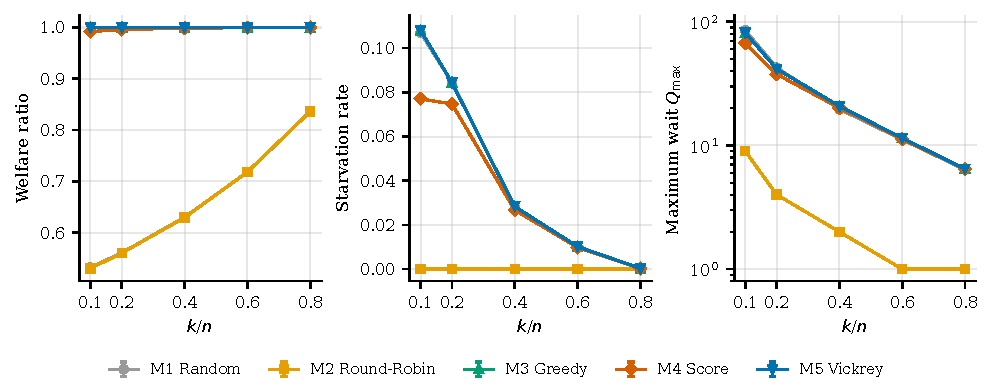
\includegraphics[width=\textwidth]{fig_e1}
\caption{E1: welfare ratio, starvation rate and maximum wait against $k/n$ with 95\% intervals. The curves of M3 and M5 coincide, M1 and M2 coincide in welfare, and M1 is hidden behind M3 in the other panels.}
\label{fig:e1}
\end{figure}

\paragraph{Heterogeneous users (E4).}
When half of the users draw from $\mathrm{Beta}(2,5)$ and half from $\mathrm{Beta}(5,2)$, Greedy and Vickrey send almost every GPU to the high-value group, and both fairness indices fall to about 0.51 (Table~\ref{tab:e4}).
The maximum wait of Greedy in this population is 974.6 rounds out of $T=1000$.
Score keeps benefit fairness at the level of random allocation and round-robin ($\JB=0.995$) while recovering most of the welfare (0.897 against 0.581), and it has the highest Nash social welfare of the five rules (245.4 against 225.2 for round-robin and 142.1 for Greedy).
It serves the high-value group somewhat more often ($\JA=0.925$), so it trades equal service for nearly equal normalised benefit.
Round-robin has the highest $\JB$ (0.999), so equal service and equal benefit diverge only for rules that read values.

\begin{table}[!htb]
\caption{E4: heterogeneous population (half $\mathrm{Beta}(2,5)$, half $\mathrm{Beta}(5,2)$), truthful reports.}
\label{tab:e4}
\centering
\footnotesize
\setlength{\tabcolsep}{4pt}
\adjustbox{max width=\textwidth}{%
\begin{tabular}{lrrrrr}
\toprule
Mechanism & WR & $J_A$ & $J_B$ & $\mathrm{SR}_\Delta$ & NSW \\
\midrule
M1 Random & 0.581 & 0.996 & 0.995 & 0.085 & 225.1 \\
M2 Round-Robin & 0.581 & 1.000 & 0.999 & 0.000 & 225.2 \\
M3 Greedy & 1.000 & 0.507 & 0.517 & 0.480 & 142.1 \\
M4 Score ($\lambda=1$) & 0.897 & 0.925 & 0.995 & 0.098 & 245.4 \\
M5 Vickrey & 1.000 & 0.507 & 0.517 & 0.480 & 142.1 \\
\bottomrule
\end{tabular}}
\end{table}


\paragraph{Persistent demand (E5).}
With the recursion of the proposal, $v_{i,t}=\alpha v_{i,t-1}+(1-\alpha)\epsilon_{i,t}$, the welfare of random allocation and round-robin rises with $\alpha$ (0.56 to 0.85 at $\alpha=0.9$, Table~\ref{tab:e5}).
This is an artefact of the recursion, which also shrinks the spread of values by a factor of $\sqrt{(1-\alpha)/(1+\alpha)}$ and so makes users look alike; it does not measure persistence.
A marginal-preserving copula keeps the welfare of the report-blind rules flat at 0.56.
Under either construction, Greedy and Vickrey keep $\WR=1$ but monopolise service: $\JA$ falls from 0.996 to 0.957, $\Qmax$ rises from 41.7 to 204.7 (210.4 under the copula), and the starvation rate rises from 8.4\% to 49.2\% (49.8\%).
Score keeps $\JA\ge 0.995$ and welfare near 0.97 and starves less than Greedy (37.7\% under the proposal recursion and 44.5\% under the copula, against about 49\%), but far more than random allocation (8.5\%) or round-robin (0\%).
A penalty on cumulative allocations equalises totals and not waiting times.
The proposal recursion understates the effect of persistence on Score.

\begin{table}[!htb]
\caption{E5 at $\alpha=0.9$, truthful reports. The proposal recursion shrinks the value spread; the copula control preserves the marginal distribution.}
\label{tab:e5}
\centering
\footnotesize
\setlength{\tabcolsep}{4pt}
\adjustbox{max width=\textwidth}{%
\begin{tabular}{lrrrrrrrr}
\toprule
 & \multicolumn{4}{c}{Proposal recursion} & \multicolumn{4}{c}{Copula control} \\
\cmidrule(lr){2-5}\cmidrule(lr){6-9}
Mechanism & WR & $J_A$ & $Q_{\max}$ & $\mathrm{SR}_\Delta$ & WR & $J_A$ & $Q_{\max}$ & $\mathrm{SR}_\Delta$ \\
\midrule
M1 Random & 0.846 & 0.996 & 42.7 & 0.085 & 0.561 & 0.996 & 42.7 & 0.085 \\
M2 Round-Robin & 0.846 & 1.000 & 4.0 & 0.000 & 0.561 & 1.000 & 4.0 & 0.000 \\
M3 Greedy & 1.000 & 0.957 & 204.7 & 0.492 & 1.000 & 0.957 & 210.4 & 0.498 \\
M4 Score ($\lambda=1$) & 0.971 & 0.998 & 130.3 & 0.377 & 0.969 & 0.995 & 165.7 & 0.445 \\
M5 Vickrey & 1.000 & 0.957 & 204.7 & 0.492 & 1.000 & 0.957 & 210.4 & 0.498 \\
\bottomrule
\end{tabular}}
\end{table}


\paragraph{Scalability (E6).}
Time per round grows gently with $n$, from 22 to 54 microseconds at $n=10$ to 40 to 111 microseconds at $n=500$, depending on the mechanism (Figure~\ref{fig:e6}); round-robin is the fastest and Greedy and Score the slowest at $n=500$.
Peak traced memory, measured with \texttt{tracemalloc} over the seed package and the full $T=1000$ simulation, grows linearly from 0.5~MiB at $n=10$ to 11.7~MiB at $n=500$ and is the same for all mechanisms to within 0.1\%.
Timings depend on the machine.

\begin{figure}[!htb]
\centering
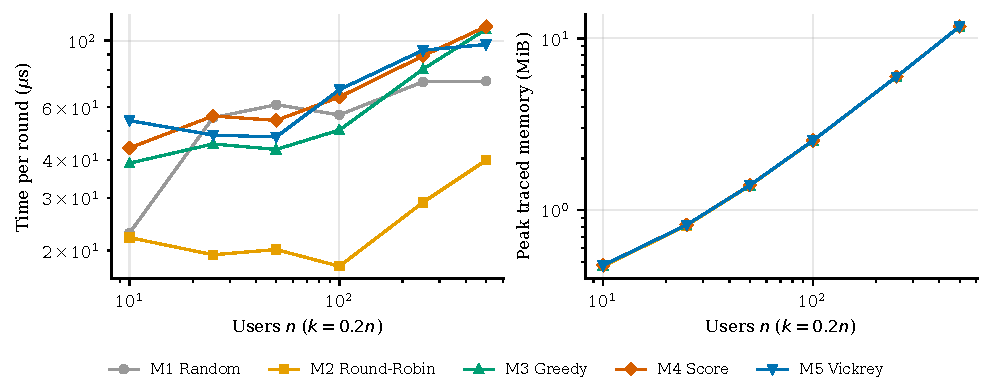
\includegraphics[width=\textwidth]{fig_e6}
\caption{E6: time per simulated round and peak traced memory against the number of users. The memory curves of the five mechanisms coincide.}
\label{fig:e6}
\end{figure}

\subsection{Strategic behaviour of the baseline rules}

\paragraph{The $\lambda$ sweep (E2).}
Table~\ref{tab:e2} and Figure~\ref{fig:lambda} show the effect of the history penalty when a quarter of the users inflate with $c=2$.
Greedy is extremely manipulable: one inflating user gains 305.7 utility units over the episode, and every focal user gains.
The penalty reduces the individual gain monotonically in $\lambda$, and welfare under manipulation rises from 0.893 at $\lambda=0$ to about 0.96 at $\lambda=1$ while $\JA$ approaches one.
At $\lambda=1$ the coalition gain is negative ($-3.2$), but one user who inflates alone still gains $+3.5$ [2.7, 4.3], and 82\% of focal users gain.
The coalition number is negative only because the twelve inflating users displace one another.
The individual gain turns negative between $\lambda=1$ and $\lambda=2$.
The Pareto filter over ($\WR$, $\JA$, $\SR$, $\Muni$) keeps round-robin, Vickrey and M4 at $\lambda\in\{1,2,5\}$; random allocation, Greedy and M4 at $\lambda\le 0.5$ are dominated.

\begin{table}[!htb]
\caption{E2: $\lambda$ sweep with $\rho=0.25$ of users using capped exaggeration with $c=2$. The last column marks settings that are non-dominated on (WR, $J_A$, $\mathrm{SR}_\Delta$, $M_{\mathrm{uni}}$).}
\label{tab:e2}
\centering
\footnotesize
\setlength{\tabcolsep}{4pt}
\adjustbox{max width=\textwidth}{%
\begin{tabular}{lrrrrlrc}
\toprule
Mechanism & WR & $J_A$ & $\mathrm{SR}_\Delta$ & Coalition $M$ & Unilateral $M_{\mathrm{uni}}$ [95\% CI] & Frac. gaining & Pareto \\
\midrule
M1 Random & 0.561 & 0.996 & 0.085 & 0.0 & 0.0 [0.0, 0.0] & 0.00 &  \\
M2 Round-Robin & 0.560 & 1.000 & 0.000 & 0.0 & 0.0 [0.0, 0.0] & 0.00 & $\checkmark$ \\
M3 Greedy & 0.893 & 0.506 & 0.270 & +220.1 & +305.7 [303.7, 307.4] & 1.00 &  \\
M5 Vickrey & 0.893 & 0.506 & 0.270 & $-$117.4 & $-$101.8 [$-$102.6, $-$101.1] & 0.00 & $\checkmark$ \\
\midrule
M4 Score ($\lambda=0$) & 0.893 & 0.506 & 0.270 & +220.1 & +305.7 [303.7, 307.4] & 1.00 &  \\
M4 Score ($\lambda=0.25$) & 0.953 & 0.898 & 0.104 & +59.4 & +86.8 [86.0, 87.5] & 1.00 &  \\
M4 Score ($\lambda=0.5$) & 0.959 & 0.967 & 0.082 & +19.7 & +33.7 [32.8, 34.6] & 1.00 &  \\
M4 Score ($\lambda=1$) & 0.960 & 0.991 & 0.069 & $-$3.2 & +3.5 [2.7, 4.3] & 0.82 & $\checkmark$ \\
M4 Score ($\lambda=2$) & 0.957 & 0.997 & 0.060 & $-$15.3 & $-$12.5 [$-$13.1, $-$11.8] & 0.00 & $\checkmark$ \\
M4 Score ($\lambda=5$) & 0.949 & 1.000 & 0.045 & $-$22.2 & $-$21.3 [$-$21.7, $-$20.9] & 0.00 & $\checkmark$ \\
\bottomrule
\end{tabular}}
\end{table}


\begin{figure}[!htb]
\centering
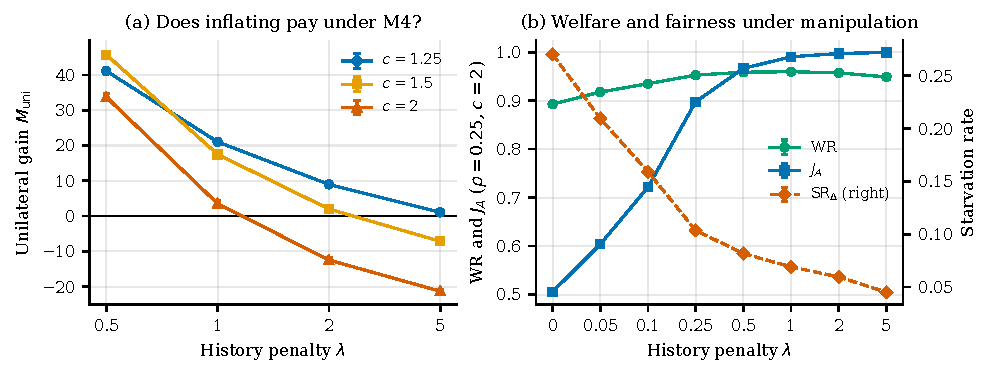
\includegraphics[width=\textwidth]{fig_lambda}
\caption{(a) Unilateral gain of M4 against capped exaggeration of three strengths (E7). (b) Welfare, allocation fairness and starvation against $\lambda$ with a quarter of users using $c=2$ (E2). Bars are 95\% intervals.}
\label{fig:lambda}
\end{figure}

\paragraph{Dependence on the size of the lie (E7).}
The threshold at $c=2$ does not generalise (Table~\ref{tab:e7}).
At $\lambda=2$ inflating stops paying for $c=2$ ($-12.5$), is marginal for $c=1.5$ (+2.0, and 78\% of focal users still gain), and still pays for $c=1.25$ (+9.0, with every focal user gaining).
At $\lambda=5$, the largest value tested, mild exaggeration still gains slightly (+1.1, with 77\% of focal users gaining).
The penalty needed to deter a lie therefore grows as the lie gets milder.
Vickrey deters every lie at every size.
The simple statement that Score with $\lambda\approx 2$ replaces Vickrey without money holds only for $c=2$.

\begin{table}[!htb]
\caption{E7: unilateral gain $M_{\mathrm{uni}}$ [95\% CI] from capped exaggeration with factor $c$ ($\rho=0.25$); the fraction of focal users who gain is in parentheses.}
\label{tab:e7}
\centering
\footnotesize
\setlength{\tabcolsep}{4pt}
\adjustbox{max width=\textwidth}{%
\begin{tabular}{lccc}
\toprule
Mechanism & $c=1.25$ & $c=1.5$ & $c=2$ \\
\midrule
M3 Greedy & +126.7 [124.9, 128.5] (1.00) & +208.7 [206.5, 210.8] (1.00) & +305.7 [303.7, 307.4] (1.00) \\
\midrule
M4 Score ($\lambda=0.5$) & +41.1 [40.7, 41.6] (1.00) & +45.7 [45.1, 46.4] (1.00) & +33.7 [32.8, 34.6] (1.00) \\
M4 Score ($\lambda=1$) & +21.0 [20.7, 21.4] (1.00) & +17.5 [16.9, 18.1] (1.00) & +3.5 [2.7, 4.3] (0.82) \\
M4 Score ($\lambda=2$) & +9.0 [8.7, 9.3] (1.00) & +2.0 [1.5, 2.5] (0.78) & $-$12.5 [$-$13.1, $-$11.8] (0.00) \\
M4 Score ($\lambda=5$) & +1.1 [0.8, 1.3] (0.77) & $-$7.2 [$-$7.5, $-$6.8] (0.00) & $-$21.3 [$-$21.7, $-$20.9] (0.00) \\
\midrule
M5 Vickrey & $-$14.0 [$-$14.3, $-$13.8] (0.00) & $-$41.8 [$-$42.2, $-$41.3] (0.00) & $-$101.8 [$-$102.6, $-$101.1] (0.00) \\
\bottomrule
\end{tabular}}
\end{table}


\paragraph{Strategic fraction and attack type (E3).}
Random allocation and round-robin are unaffected by every attack: all gains and prices of strategy are exactly zero.
Under Greedy, inflating always pays individually, even when everyone already inflates (+148.5 for $c=2$ at $\rho=1$), and maximum claim at $\rho\ge 0.25$ drops welfare to the random level (0.561), with $\JA$ falling to 0.24 at $\rho=0.25$.
Under Vickrey inflating never pays, in line with per-round DSIC, so the welfare collapse under maximum claim needs users to act against their own interest. It is a stress test, not an equilibrium outcome.
Under Score, maximum claim is unprofitable at every $\rho$ ($-47$ to $-54$), and capped exaggeration pays a little when few others inflate ($+5.5$ at $\rho=0$, $+3.5$ at $0.25$), is indistinguishable from zero at $\rho=0.5$ and is negative at $\rho=1$ (Table~\ref{tab:e3}).
Welfare under attack degrades gracefully, and $\JA$ stays near 0.99 or higher for capped exaggeration.

\begin{table}[!htb]
\caption{E3: unilateral gain by strategic fraction $\rho$ and the welfare ratio and price of strategy at $\rho=0.25$. M1 and M2 have zero gain and zero PoS in every cell.}
\label{tab:e3}
\centering
\footnotesize
\setlength{\tabcolsep}{4pt}
\adjustbox{max width=\textwidth}{%
\begin{tabular}{llrrrrr}
\toprule
Mechanism & Attack & $M_{\mathrm{uni}}$ $\rho=0$ & $\rho=0.25$ & $\rho=1$ & WR ($\rho=0.25$) & PoS ($\rho=0.25$) \\
\midrule
M3 Greedy & cap 2 & +241.3 & +305.7 & +148.5 & 0.893 & 0.107 \\
M3 Greedy & max claim & +321.6 & +417.6 & +99.0 & 0.561 & 0.439 \\
\midrule
M4 Score ($\lambda=1$) & cap 2 & +5.5 & +3.5 & $-$2.7 & 0.960 & 0.036 \\
M4 Score ($\lambda=1$) & max claim & $-$47.4 & $-$53.6 & $-$52.6 & 0.883 & 0.113 \\
\midrule
M5 Vickrey & cap 2 & $-$80.5 & $-$101.8 & $-$49.6 & 0.893 & 0.107 \\
M5 Vickrey & max claim & $-$320.9 & $-$416.1 & $-$99.2 & 0.561 & 0.439 \\
\bottomrule
\end{tabular}}
\end{table}


\paragraph{Does timing pay (E8).}
The proposal's second hypothesis suggests that a larger $\lambda$ may reward strategic timing, because current service changes future scores.
We tested rules that inflate only while the user's own allocation count is low.
Timing never beats indiscriminate inflation where inflation is profitable (Table~\ref{tab:e8}), and its own gain is at most $+5.6$ for M4 across the full grid (which also includes $\lambda=0.5$) and about zero or negative for $\lambda\ge 2$.
For M4, timing beats always-inflating only at $c=2$ and $\lambda\ge 2$, where always-inflating has become expensive and timing means lying less.
The hypothesis in its simple form is not supported, since the value of this kind of timing does not rise with $\lambda$.

\begin{table}[!htb]
\caption{E8: unilateral gain of inflating always versus inflating only while the user's own allocation count is at most the population mean, 25th or 75th percentile ($\rho=0.25$).}
\label{tab:e8}
\centering
\footnotesize
\setlength{\tabcolsep}{4pt}
\adjustbox{max width=\textwidth}{%
\begin{tabular}{llrrrr}
\toprule
Mechanism & $c$ & Always & Timed (mean) & Timed (q25) & Timed (q75) \\
\midrule
M4 Score ($\lambda=1$) & 1.25 & +21.0 & +0.7 & +0.2 & +2.6 \\
M4 Score ($\lambda=1$) & 2 & +3.5 & $-$2.8 & $-$2.4 & $-$5.0 \\
\midrule
M4 Score ($\lambda=2$) & 1.25 & +9.0 & $-$0.5 & $-$0.7 & +0.4 \\
M4 Score ($\lambda=2$) & 2 & $-$12.5 & $-$5.4 & $-$4.5 & $-$10.3 \\
\midrule
M4 Score ($\lambda=5$) & 1.25 & +1.1 & $-$2.2 & $-$1.9 & $-$1.9 \\
M4 Score ($\lambda=5$) & 2 & $-$21.3 & $-$9.1 & $-$8.0 & $-$16.5 \\
\bottomrule
\end{tabular}}
\end{table}


\paragraph{Far-sighted attackers (E3b and E3c).}
With the five-round horizon of the proposal, the rollout attack finds a stronger attack than capped exaggeration against Greedy, rediscovers truth-telling against Vickrey, and finds no profitable attack against Score (Table~\ref{tab:e3b}).
The last result is a horizon artefact.
Five rounds see the immediate gain from reporting $\vmax$ but not the history penalty that persists afterwards, so the attacker over-inflates and loses.
Lengthening the horizon changes the conclusion (Table~\ref{tab:e3c}, Figure~\ref{fig:rollout}).
The gain rises with the horizon, and its interval lies above zero from $H=40$.
At $\lambda=2$ it plateaus near $+3.2$ and beats both capped rules, including $c=1.25$, and at $\lambda=1$ it is still rising at $H=80$ ($+7.2$).
The mean report converges to the true value, so the attack is selective: it inflates in a few well-chosen rounds and not in every round.
A penalty of $\lambda=2$ stops the simple lie but not a planner, and this is a lower bound on what a sophisticated attacker can do.
These results come from the historical checkpoint described in Section~\ref{sec:attackers}.

\begin{table}[!htb]
\caption{E3b (historical checkpoint): proposal-style rollout attack with $H=5$ ($n=10$, $T=500$). Entries are the mean gain of the focal user.}
\label{tab:e3b}
\centering
\footnotesize
\setlength{\tabcolsep}{4pt}
\adjustbox{max width=\textwidth}{%
\begin{tabular}{lrrrrr}
\toprule
Mechanism & Rollout (truthful opp.) & Cap 2 & Rollout (cap-2 opp.) & Cap 2 & Share at $v_{\max}$ \\
\midrule
M3 Greedy & +164.8 & +123.8 & +98.0 & +73.1 & 1.00 \\
M4 Score ($\lambda=1$) & $-$18.3 & +0.9 & $-$22.2 & $-$1.8 & 0.95 \\
M4 Score ($\lambda=2$) & $-$23.3 & $-$6.2 & $-$24.2 & $-$6.8 & 0.92 \\
M5 Vickrey & $-$0.2 & $-$41.6 & 0.0 & $-$24.0 & 0.06 \\
\bottomrule
\end{tabular}}
\end{table}

\begin{table}[!htb]
\caption{E3c (historical checkpoint): gain of one rollout attacker against M4 with truthful opponents ($n=10$, $T=300$) as the planning horizon grows. The last two rows give the capped-exaggeration gains on the same workloads.}
\label{tab:e3c}
\centering
\footnotesize
\setlength{\tabcolsep}{4pt}
\adjustbox{max width=\textwidth}{%
\begin{tabular}{lrrrr}
\toprule
Horizon $H$ & $\lambda=1$ gain [95\% CI] & Share at $v_{\max}$ & $\lambda=2$ gain [95\% CI] & Share at $v_{\max}$ \\
\midrule
5 & $-$9.61 [$-$10.30, $-$8.90] & 0.93 & $-$12.47 [$-$13.15, $-$11.81] & 0.88 \\
10 & $-$7.04 [$-$7.69, $-$6.38] & 0.85 & $-$8.58 [$-$9.24, $-$7.94] & 0.74 \\
20 & $-$2.93 [$-$3.56, $-$2.31] & 0.72 & $-$2.68 [$-$3.24, $-$2.12] & 0.53 \\
40 & +2.97 [2.41, 3.55] & 0.52 & +3.19 [2.77, 3.62] & 0.29 \\
80 & +7.20 [6.76, 7.63] & 0.31 & +3.24 [2.77, 3.68] & 0.19 \\
\midrule
capped $c=2$ & +0.91 &  & $-$3.48 &  \\
capped $c=1.25$ & +3.88 &  & +1.29 &  \\
\bottomrule
\end{tabular}}
\end{table}


\begin{figure}[!htb]
\centering
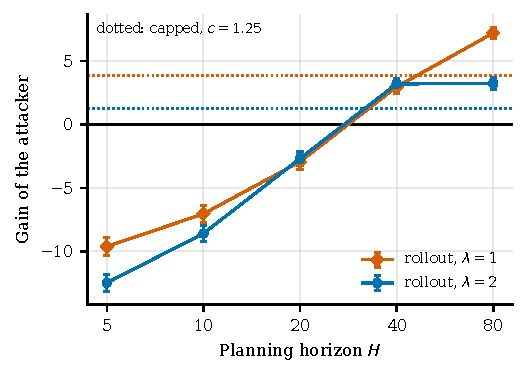
\includegraphics[width=0.58\textwidth]{fig_rollout}
\caption{E3c (historical checkpoint): gain of the rollout attacker against M4 with truthful opponents as the horizon grows. Dotted lines mark the gain of capped exaggeration with $c=1.25$ at the same $\lambda$.}
\label{fig:rollout}
\end{figure}

\subsection{The proposed mechanisms}

\paragraph{Design motivation.}
The analysis above leaves three gaps in the baselines.
A cumulative-allocation penalty does not bound waiting, it deters lying only partly, and Vickrey needs money.
M6 and M7 aim for a hard waiting bound, for lies that cost future priority, and for value-aware selection.
The default wait cap is $W=\Delta=10$.

\paragraph{Truthful behaviour (E9).}
On the base workload, M6 and M7 reach a welfare ratio of 0.942 and 0.945 against 0.996 for Score, with an observed maximum wait of 10 rounds and no starvation (Table~\ref{tab:e9}).
The wait cap has a welfare cost that depends on $W$ (Table~\ref{tab:e9w}, Figure~\ref{fig:e9}).
M7 with $W=15$ to $20$ gives welfare of 0.98 to 0.99 with observed waits of 15 to 20 rounds, against about 38 rounds for Score.
The general guarantee is $W+\lceil n/k\rceil-1$.
Under heterogeneous demand or persistent demand with a preserved value distribution, the cap forces service to low-value users, and welfare falls to between 0.72 and 0.81 against 0.90 to 0.97 for Score.
The guarantee is expensive exactly when values differ.

\begin{table}[!htb]
\caption{E9: truthful reports on the locked seeds. M6 and M7 use the wait cap $W=10$ (the default $W=\Delta$).}
\label{tab:e9}
\centering
\footnotesize
\setlength{\tabcolsep}{4pt}
\adjustbox{max width=\textwidth}{%
\begin{tabular}{llrrrr}
\toprule
Condition & Mechanism & WR & $J_B$ & $Q_{\max}$ & $\mathrm{SR}_\Delta$ \\
\midrule
base & M3 Greedy & 1.000 & 0.996 & 41.7 & 0.084 \\
 & M4 Score ($\lambda=1$) & 0.996 & 0.999 & 37.7 & 0.075 \\
 & M6 Karma-Cap & 0.942 & 1.000 & 10.0 & 0.000 \\
 & M7 Rank-Cap & 0.945 & 0.999 & 10.0 & 0.000 \\
\midrule
scarce ($k/n=0.1$) & M3 Greedy & 1.000 & 0.991 & 81.7 & 0.108 \\
 & M4 Score ($\lambda=1$) & 0.992 & 0.999 & 67.1 & 0.077 \\
 & M6 Karma-Cap & 0.933 & 0.999 & 20.4 & 0.000 \\
 & M7 Rank-Cap & 0.930 & 0.999 & 20.0 & 0.000 \\
\midrule
mixed groups & M3 Greedy & 1.000 & 0.517 & 974.6 & 0.480 \\
 & M4 Score ($\lambda=1$) & 0.897 & 0.995 & 49.8 & 0.098 \\
 & M6 Karma-Cap & 0.722 & 0.940 & 11.9 & 0.000 \\
 & M7 Rank-Cap & 0.804 & 0.971 & 10.0 & 0.000 \\
\midrule
persistent (copula, $\alpha=0.9$) & M3 Greedy & 1.000 & 0.954 & 210.4 & 0.498 \\
 & M4 Score ($\lambda=1$) & 0.969 & 0.994 & 165.7 & 0.445 \\
 & M6 Karma-Cap & 0.752 & 0.998 & 11.1 & 0.000 \\
 & M7 Rank-Cap & 0.813 & 0.995 & 10.0 & 0.000 \\
\bottomrule
\end{tabular}}
\end{table}

\begin{table}[!htb]
\caption{E9: truthful welfare ratio as the wait cap $W$ varies ($n=50$, $k=10$).}
\label{tab:e9w}
\centering
\footnotesize
\setlength{\tabcolsep}{4pt}
\adjustbox{max width=\textwidth}{%
\begin{tabular}{lccccc}
\toprule
Mechanism & $W=6$ & $W=10$ & $W=15$ & $W=20$ & $W=30$ \\
\midrule
M6 Karma-Cap & 0.817 & 0.942 & 0.969 & 0.973 & 0.974 \\
M7 Rank-Cap & 0.813 & 0.945 & 0.981 & 0.990 & 0.993 \\
\bottomrule
\end{tabular}}
\end{table}


\begin{figure}[!htb]
\centering
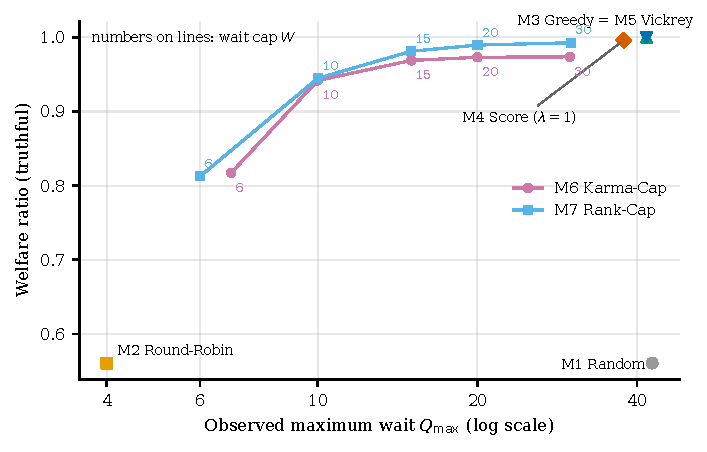
\includegraphics[width=0.78\textwidth]{fig_e9}
\caption{E9: truthful welfare ratio against the observed maximum wait. M6 and M7 trace a frontier as the wait cap $W$ varies; M3 and M5 coincide.}
\label{fig:e9}
\end{figure}

\paragraph{Individual gain from lying (E10).}
Table~\ref{tab:e10} gives the unilateral gain from each scripted lie.
At $\rho=0.25$ Karma-Cap has a negative mean gain for every tested lie, including mild $c=1.25$ and timed lies, although some focal users still gain.
Rank-Cap has a negative mean gain for all but the mildest lie ($c=1.25$, $+1.8$, against $+21.0$ for Score at $\lambda=1$).
Karma-Cap's deterrence reverses when everyone else already lies: at $\rho=1$ the gain is $+46.1$ for $c=2$ and every focal user gains.
Truthful reporting therefore does not remain an equilibrium of Karma-Cap.
Score, Vickrey and Rank-Cap stay negative at $\rho=1$.
The karma supply matters, since with a larger initial balance timed lies pay again, and a smaller supply deters more and is less efficient.
Welfare under attack ($c=2$, $\rho=0.25$) is 0.903 for Karma-Cap, 0.921 for Rank-Cap, 0.960 for Score and 0.893 for Greedy and Vickrey.

\begin{table}[!htb]
\caption{E10: unilateral gain $M_{\mathrm{uni}}$ from each scripted lie at $\rho=0.25$ (last two columns: $\rho=1$).}
\label{tab:e10}
\centering
\footnotesize
\setlength{\tabcolsep}{4pt}
\adjustbox{max width=\textwidth}{%
\begin{tabular}{lrrrrrrr}
\toprule
Mechanism & $c=1.25$ & $c=1.5$ & $c=2$ & max & timed 1.25 & $\rho{=}1$, $c{=}2$ & $\rho{=}1$, max \\
\midrule
M3 Greedy & +126.7 & +208.7 & +305.7 & +417.6 & +7.5 & +148.5 & +99.0 \\
\midrule
M4 ($\lambda=1$) & +21.0 & +17.5 & +3.5 & $-$53.6 & +0.7 & $-$2.7 & $-$52.6 \\
M4 ($\lambda=2$) & +9.0 & +2.0 & $-$12.5 & $-$65.4 & $-$0.5 & $-$13.7 & $-$63.3 \\
M5 Vickrey & $-$14.0 & $-$41.8 & $-$101.8 & $-$416.1 & $-$0.9 & $-$49.6 & $-$99.2 \\
\midrule
M6 Karma-Cap & $-$8.3 & $-$17.1 & $-$29.1 & $-$69.0 & $-$2.3 & +46.1 & +6.1 \\
M7 Rank-Cap & +1.8 & $-$10.6 & $-$35.9 & $-$113.9 & $-$1.3 & $-$34.1 & $-$141.8 \\
\bottomrule
\end{tabular}}
\end{table}


\paragraph{Far-sighted attacker (E11).}
In the historical results neither proposed mechanism has a positive mean attack gain, whereas Score is attacked from $H=40$ (Table~\ref{tab:e11}).
The loss under Karma-Cap is flat at about $-2.2$, but the loss under Rank-Cap shrinks with the horizon ($-20.9$, $-11.9$, $-4.4$), so a longer horizon could turn it positive.
In that rollout the rank quantiles are frozen at the current round, which favours Rank-Cap, and the corrected attacker of Section~\ref{sec:course} shows that this matters.

\begin{table}[!htb]
\caption{E11 (historical checkpoint): mean gain of the rollout attacker ($n=10$, $T=300$, truthful opponents). Score columns repeat E3c.}
\label{tab:e11}
\centering
\footnotesize
\setlength{\tabcolsep}{4pt}
\adjustbox{max width=\textwidth}{%
\begin{tabular}{lrrrr}
\toprule
Horizon $H$ & M6 Karma-Cap & M7 Rank-Cap & M4 ($\lambda=1$) & M4 ($\lambda=2$) \\
\midrule
5 & $-$7.05 & $-$20.94 & $-$9.61 & $-$12.47 \\
40 & $-$2.32 & $-$11.85 & +2.97 & +3.19 \\
80 & $-$2.17 & $-$4.41 & +7.20 & +3.24 \\
\bottomrule
\end{tabular}}
\end{table}


\subsection{Component, adaptive and benchmark studies}
\label{sec:course}

The next four studies use the 30 held-out seeds.

\paragraph{Cap and incentive components (E12).}
A cap alone does not deter mild exaggeration (Table~\ref{tab:e12}).
At $W=10$, $c=1.25$ and $\rho=0.25$, the mean unilateral gain is $+20.8$ for Score-Cap, $-8.2$ for Karma-Cap and $+2.2$ for Rank-Cap over 1000 rounds.
Score-Cap and Score differ little in gain ($+20.8$ against $+21.0$), so the cap contributes almost nothing to deterrence, and the lower gain of Karma-Cap comes from its incentive component.
Adding the cap costs welfare in every family (about 0.05 for Score and Rank, and 0.03 for Karma, Table~\ref{tab:e12c}).
Karma-Cap and Rank-Cap differ from Score-Cap at the same $W$ by $-28.9$ and $-18.6$ in gain.
The population reversal is also visible: at $\rho=1$ with $c=2$ Karma-Cap gains $+46.1$ and Score-Cap $+3.9$, while Rank-Cap stays at $-34.3$.
A reduction in average gain is distinct from eliminating gains for every user, and truthful-row gains are zero by construction.

\begin{table}[!htb]
\caption{E12 (fresh held-out seeds): cap and incentive components on the homogeneous workload. Capped rules use $W=10$. ``Frac.'' is the fraction of focal users with a positive gain.}
\label{tab:e12}
\centering
\footnotesize
\setlength{\tabcolsep}{4pt}
\adjustbox{max width=\textwidth}{%
\begin{tabular}{lrrlrlr}
\toprule
Rule & WR (truthful) & $Q_{\max}$ & Gain, $c=1.25$, $\rho=0.25$ & Frac. & Gain, $c=2$, $\rho=1$ & Frac. \\
\midrule
Score & 0.996 & 39.2 & +21.0 [20.5, 21.4] & 1.00 & $-$3.1 [$-$3.7, $-$2.5] & 0.23 \\
Score-Cap & 0.948 & 10.0 & +20.8 [20.3, 21.2] & 1.00 & +3.9 [3.1, 4.7] & 0.84 \\
\midrule
Karma & 0.974 & 36.0 & $-$13.7 [$-$14.1, $-$13.3] & 0.00 & +29.4 [28.8, 30.0] & 1.00 \\
Karma-Cap & 0.941 & 10.0 & $-$8.2 [$-$8.5, $-$7.9] & 0.00 & +46.1 [45.4, 46.7] & 1.00 \\
\midrule
Rank & 0.993 & 39.5 & +2.5 [2.3, 2.7] & 0.91 & $-$37.4 [$-$38.3, $-$36.6] & 0.00 \\
Rank-Cap & 0.945 & 10.0 & +2.2 [1.8, 2.5] & 0.80 & $-$34.3 [$-$35.3, $-$33.5] & 0.00 \\
\bottomrule
\end{tabular}}
\end{table}

\begin{table}[!htb]
\caption{E12: differences of means. The first three rows isolate adding the cap; the last two compare incentive components at the same wait cap. Paired intervals are in the saved \texttt{paired.json}.}
\label{tab:e12c}
\centering
\footnotesize
\setlength{\tabcolsep}{4pt}
\adjustbox{max width=\textwidth}{%
\begin{tabular}{lrr}
\toprule
Comparison ($c=1.25$, $\rho=0.25$) & WR difference & Gain difference \\
\midrule
Score-Cap minus Score & $-$0.049 & $-$0.19 \\
Karma-Cap minus Karma & $-$0.026 & +5.51 \\
Rank-Cap minus Rank & $-$0.049 & $-$0.33 \\
\midrule
Karma-Cap minus Score-Cap & $-$0.013 & $-$28.93 \\
Rank-Cap minus Score-Cap & $-$0.001 & $-$18.61 \\
\bottomrule
\end{tabular}}
\end{table}


\paragraph{Adaptive policy choice (E13).}
When users choose among the eight scripted policies by best response, Vickrey converges to all-truthful play, while Greedy converges to maximum claims and welfare falls to 0.643 (Table~\ref{tab:e13}).
Score converges to mild exaggeration with welfare 0.976.
For the capped rules the four-sweep limit is reached with residual incentives on the training workloads.
On the held-out seeds every regret band includes zero, so the positive point estimates do not establish positive expected regret after accounting for all inspected switches.
A sweep limit with residual training regret nevertheless prevents an equilibrium claim for the capped rules.
The two starting profiles do not exhaust the basins of attraction.

\begin{table}[!htb]
\caption{E13: adaptive finite-policy populations ($n=6$, $k=2$, $T=120$). Regret is the largest seed-averaged gain from any single policy switch, with a simultaneous bootstrap band.}
\label{tab:e13}
\centering
\footnotesize
\setlength{\tabcolsep}{4pt}
\adjustbox{max width=\textwidth}{%
\begin{tabular}{lllcrrrr}
\toprule
Start & Rule & Training & Sweeps & WR & Mean utility & Regret [band] & Truthful \\
\midrule
truthful & Greedy & converged & 2 & 0.643 & 20.20 & 0.00 [0.00, 1.55] & 0.00 \\
 & Score & converged & 4 & 0.976 & 30.67 & 0.17 [0.00, 1.12] & 0.00 \\
 & Score-Cap & sweep limit & 4 & 0.948 & 29.80 & 0.40 [0.00, 1.29] & 0.00 \\
 & Vickrey & converged & 1 & 1.000 & 8.38 & 0.00 [0.00, 1.36] & 1.00 \\
 & Karma-Cap & sweep limit & 4 & 0.954 & 29.99 & 0.58 [0.00, 1.50] & 0.00 \\
 & Rank-Cap & sweep limit & 4 & 0.948 & 29.78 & 0.63 [0.00, 1.49] & 0.33 \\
\midrule
cap 2 & Greedy & converged & 2 & 0.643 & 20.20 & 0.00 [0.00, 1.55] & 0.00 \\
 & Score & converged & 4 & 0.976 & 30.67 & 0.17 [0.00, 1.12] & 0.00 \\
 & Score-Cap & sweep limit & 4 & 0.952 & 29.92 & 0.62 [0.00, 1.51] & 0.00 \\
 & Vickrey & converged & 2 & 1.000 & 8.38 & 0.00 [0.00, 1.36] & 1.00 \\
 & Karma-Cap & sweep limit & 4 & 0.936 & 29.43 & 0.80 [0.00, 1.83] & 0.00 \\
 & Rank-Cap & sweep limit & 4 & 0.948 & 29.78 & 0.63 [0.00, 1.49] & 0.33 \\
\bottomrule
\end{tabular}}
\end{table}


\paragraph{Welfare under the same service requirement (E14).}
All 270 small oracle instances are solved to certified optimality.
At $W=6$ (so that $B=8$), Score-Cap reaches about 92\% of the constrained optimum under heterogeneous demand, against about 83\% and 82\% for Karma-Cap and Rank-Cap (Table~\ref{tab:e14}, Figure~\ref{fig:e14}).
The service requirement itself costs little on the base workload (0.002 of oracle welfare) and more under heterogeneous (0.049) and persistent (0.054) demand.
The remaining loss is larger and varies by rule, from 0.029 for Karma-Cap on the base workload to 0.201 for Rank-Cap under persistent demand.
Welfare loss therefore extends beyond what the service requirement forces, and the part that depends on the rule is largest for the incentive components designed for deterrence.
The oracle uses future information and the instances are small, so these are bounds on the online information cost and not claims that an online rule can attain the oracle.

\begin{table}[!htb]
\caption{E14 at $W=6$ ($n=6$, $k=2$, $T=40$): welfare of each online rule as a fraction of the constrained offline optimum. ``Optimal'' is the fraction of oracle solves certified optimal.}
\label{tab:e14}
\centering
\footnotesize
\setlength{\tabcolsep}{4pt}
\adjustbox{max width=\textwidth}{%
\begin{tabular}{llrlrrr}
\toprule
Demand & Rule & $B$ & Efficiency [95\% CI] & Service loss & Remaining loss & Optimal \\
\midrule
base & Score-Cap & 8 & 0.969 [0.964, 0.973] & 0.002 & 0.031 & 1.00 \\
 & Karma-Cap & 8 & 0.971 [0.967, 0.975] & 0.002 & 0.029 & 1.00 \\
 & Rank-Cap & 8 & 0.928 [0.921, 0.935] & 0.002 & 0.071 & 1.00 \\
\midrule
mixed & Score-Cap & 8 & 0.917 [0.912, 0.921] & 0.049 & 0.079 & 1.00 \\
 & Karma-Cap & 8 & 0.832 [0.826, 0.838] & 0.049 & 0.160 & 1.00 \\
 & Rank-Cap & 8 & 0.824 [0.815, 0.832] & 0.049 & 0.168 & 1.00 \\
\midrule
persistent & Score-Cap & 8 & 0.886 [0.880, 0.892] & 0.054 & 0.108 & 1.00 \\
 & Karma-Cap & 8 & 0.865 [0.855, 0.875] & 0.054 & 0.128 & 1.00 \\
 & Rank-Cap & 8 & 0.787 [0.770, 0.804] & 0.054 & 0.201 & 1.00 \\
\bottomrule
\end{tabular}}
\end{table}


\begin{figure}[!htb]
\centering
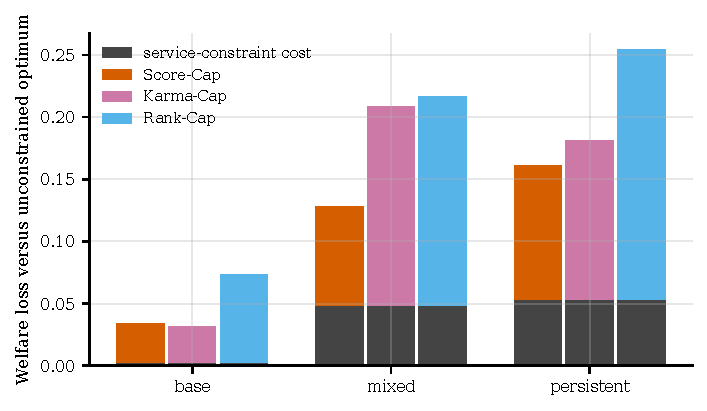
\includegraphics[width=0.78\textwidth]{fig_e14}
\caption{E14: welfare loss against the unconstrained optimum at $W=6$, split into the cost of the service requirement (the same for all rules) and the remaining loss of each online rule.}
\label{fig:e14}
\end{figure}

\paragraph{Planning attacks and computation budgets (E15).}
At the largest budget ($H=40$, 80 sampled futures per candidate) the corrected planning attacker gains $+39.6$ against Greedy, $+3.5$ against Score, $+2.2$ against Score with $\lambda=2$, $+2.6$ against Score-Cap and $+2.6$ [2.2, 3.0] against Rank-Cap with updating histories (Table~\ref{tab:e15}).
It does not profit against Vickrey (gain zero, truthful reports) or against Karma-Cap ($-0.3$ [$-0.8$, 0.2]).
With frozen rank histories the same attacker loses on Rank-Cap ($-0.9$), so the earlier negative result for Rank-Cap came from the frozen-history approximation.
The paired updating-minus-frozen difference is $+3.50$ [2.75, 4.33].
A positive gain with an interval above zero supports a profitable deviation in this workload model, whereas a negative gain only means that this particular attacker failed.
Rank-Cap is therefore vulnerable to history-aware planning even though pure rank normalisation is invariant to fixed monotone distortions.

\begin{table}[!htb]
\caption{E15 at the largest budget ($H=40$, 80 Monte Carlo futures per candidate; $n=10$, $k=2$, $T=120$): gain of the planning attacker.}
\label{tab:e15}
\centering
\footnotesize
\setlength{\tabcolsep}{4pt}
\adjustbox{max width=\textwidth}{%
\begin{tabular}{llrr}
\toprule
Rule & History model & Focal gain [95\% CI] & Truthful share \\
\midrule
Greedy & exact & +39.64 [38.78, 40.53] & 0.02 \\
Score & exact & +3.47 [3.07, 3.88] & 0.38 \\
Score ($\lambda=2$) & exact & +2.24 [1.95, 2.52] & 0.45 \\
Score-Cap & exact & +2.60 [2.29, 2.94] & 0.36 \\
Vickrey & exact & 0.00 [0.00, 0.00] & 1.00 \\
Karma-Cap & exact & $-$0.32 [$-$0.80, 0.16] & 0.41 \\
\midrule
Rank-Cap & updating & +2.58 [2.19, 2.98] & 0.36 \\
Rank-Cap & frozen & $-$0.92 [$-$1.80, $-$0.09] & 0.31 \\
\bottomrule
\end{tabular}}
\end{table}


\subsection{Why the mechanisms fail}

\paragraph{Rank-Cap and report history (E16).}
We decompose the gain of the updating attacker into forced-service and auction-service parts and replay its report sequence against a truthful reference ledger (Table~\ref{tab:e16}).
Replacing the attacked ledger with truthful reference values lowers the fixed-sequence gain from $+2.58$ to $+1.27$, so changing the report history contributes $+1.31$ [0.88, 1.73].
The attack still profits with a truthful reference, so part of its benefit comes from the current report and allocation effects and not from the ledger.
For a fixed current query $z$, replacing one past truthful report $v$ by $r$ in a ledger of size $m$ changes the empirical rank by $([r<z]+\tfrac12[r=z]-[v<z]-\tfrac12[v=z])/(m+1)$.
Understating raises the future rank for $r<z<v$, and overstating lowers it for $v<z<r$.
The updating planner exaggerates less often than the frozen planner (32\% against 54\% of rounds) and understates on relatively high values, so the trace does not support a simple rule of sacrificing only low-value rounds to build a favourable reference.
The decomposition holds the attacker's reports fixed and does not reoptimise, so it is not an additive decomposition of incentives.
The first-seed ledger effect is $-0.95$, against $+1.31$ in aggregate, which illustrates variation across seeds.

\begin{table}[!htb]
\caption{E16: Rank-Cap attacker decomposition ($n=10$, $k=2$, $T=120$, $H=40$, 80 futures).}
\label{tab:e16}
\centering
\footnotesize
\setlength{\tabcolsep}{4pt}
\adjustbox{max width=\textwidth}{%
\begin{tabular}{lrrrll}
\toprule
Attacker & Actual gain [CI] & Forced & Auction & Truthful-ref. replay [CI] & Actual minus replay [CI] \\
\midrule
updating & +2.58 [2.19, 2.98] & $-$0.90 & +3.49 & +1.27 [0.89, 1.65] & +1.31 [0.88, 1.73] \\
frozen & $-$0.92 [$-$1.80, $-$0.09] & $-$0.38 & $-$0.54 & +2.10 [1.54, 2.64] & $-$3.02 [$-$3.47, $-$2.58] \\
\bottomrule
\end{tabular}}
\end{table}


\paragraph{Karma-Cap and the population reversal (E17).}
For one deviator, the gain splits exactly into forced-service and auction-service benefit (Table~\ref{tab:e17}).
At $\rho=0.25$ the deviator spends about as many credits as before and ends with a lower value per service, and the auction benefit is negative.
At $\rho=1$ the deviator wins far more services (+63.4 for Karma-Cap) because the other bids are inflated too, and the auction benefit of $+67.0$ outweighs the forced-service benefit of $-20.9$.
Forced service is charged, so it does not come free.
The reversal also appears without the cap, which shows that the cap is not necessary for it.
At $\rho=1$ the deviator's bids are limited by its balance less often (14\% against 62\% at $\rho=0.25$) and its mean balance is higher, so the opportunity-cost deterrent weakens when other bids are inflated.
These diagnostics describe one policy and one population mix, and they do not characterise karma games in general.

\begin{table}[!htb]
\caption{E17: decomposition of the cap-2 deviation gain of a focal user ($n=50$, $k=10$, $T=1000$).}
\label{tab:e17}
\centering
\footnotesize
\setlength{\tabcolsep}{4pt}
\adjustbox{max width=\textwidth}{%
\begin{tabular}{llrrrrr}
\toprule
Rule & $\rho$ & Total gain [CI] & Forced & Auction & $\Delta$ services & $\Delta$ credits spent \\
\midrule
Karma & 0.25 & $-$35.82 [$-$36.22, $-$35.43] & 0.00 & $-$35.82 & +1.22 & +1.59 \\
 & 1 & +29.43 [28.85, 30.01] & 0.00 & +29.43 & +65.16 & +93.64 \\
\midrule
Karma-Cap & 0.25 & $-$29.23 [$-$29.75, $-$28.71] & $-$11.21 & $-$18.01 & +0.35 & +1.64 \\
 & 1 & +46.06 [45.40, 46.74] & $-$20.90 & +66.96 & +63.44 & +80.67 \\
\bottomrule
\end{tabular}}
\end{table}


\paragraph{Longer adaptive training (E18).}
Longer training does not resolve the residual incentives for every rule (Table~\ref{tab:e18}).
Karma-Cap reaches a training fixed point at sweep 18 from both starting profiles, whereas Score-Cap and Rank-Cap still have residual training incentives after twenty sweeps.
One four-sweep Karma-Cap profile has an independent regret band that excludes zero (1.54 [0.59, 2.50] from the all-$c{=}2$ start), and its twenty-sweep profile has regret 0.07 [0, 1.03].
A training fixed point is a restricted pure-policy equilibrium on five training traces and not dynamic strategyproofness, and an evaluation interval that contains zero does not establish positive expected regret.

\begin{table}[!htb]
\caption{E18: four versus twenty training sweeps, evaluated on 30 independent seeds. Greedy, Score and Vickrey reach a fixed point within four sweeps in every start and are omitted.}
\label{tab:e18}
\centering
\footnotesize
\setlength{\tabcolsep}{4pt}
\adjustbox{max width=\textwidth}{%
\begin{tabular}{lllllrl}
\toprule
Rule & Start & Budget & Status & Sweeps used & Training regret & Independent regret [band] \\
\midrule
Score-Cap & truthful & 4 & sweep limit & 4 & 1.163 & 0.21 [0.00, 1.11] \\
 &  & 20 & sweep limit & 20 & 0.682 & 0.66 [0.00, 1.60] \\
 & cap 2 & 4 & sweep limit & 4 & 0.694 & 0.63 [0.00, 1.61] \\
 &  & 20 & sweep limit & 20 & 0.682 & 0.66 [0.00, 1.60] \\
\midrule
Karma-Cap & truthful & 4 & sweep limit & 4 & 0.457 & 0.59 [0.00, 1.50] \\
 &  & 20 & converged & 18 & 0.000 & 0.07 [0.00, 1.03] \\
 & cap 2 & 4 & sweep limit & 4 & 0.477 & 1.54 [0.59, 2.50] \\
 &  & 20 & converged & 18 & 0.000 & 0.07 [0.00, 1.03] \\
\midrule
Rank-Cap & truthful & 4 & sweep limit & 4 & 0.620 & 0.58 [0.00, 1.47] \\
 &  & 20 & sweep limit & 20 & 0.235 & 0.27 [0.00, 1.27] \\
 & cap 2 & 4 & sweep limit & 4 & 0.620 & 0.58 [0.00, 1.47] \\
 &  & 20 & sweep limit & 20 & 0.235 & 0.27 [0.00, 1.27] \\
\bottomrule
\end{tabular}}
\end{table}


\section{Discussion}
\label{sec:discussion}

\paragraph{Hypotheses.}
We stated four hypotheses in the proposal and the evidence supports them to different degrees.
The first, that a moderate $\lambda$ reduces starvation before it costs welfare, is supported for fairness and weak for starvation.
Under i.i.d.\ truthful values Score at $\lambda=1$ reduces the starvation rate only from 8.4\% to 7.5\%, and from 49\% to 38\% under strong persistence.
Its large effect appears when users are strategic (the starvation rate falls from 27\% to 6.9\% between $\lambda=0$ and $\lambda=1$ in E2) or heterogeneous ($\JB$ rises from 0.52 to 0.995).
The second, that a larger $\lambda$ increases the value of strategic timing, is not supported for the fixed timing rules of E8 and is not refuted for planning attackers.
The third, that round-robin scores well on $\JA$ and badly on welfare but need not dominate on $\JB$, is partly supported: round-robin has the best $\JA$ and the lowest welfare, and it also has the highest $\JB$, because value-blind rules equalise expected normalised benefit.
The fourth, that Vickrey has negligible gain while Greedy and Score remain vulnerable, is supported, and Score is vulnerable more strongly than the proposal expected (mild lies, and planning attackers with long horizons).

\paragraph{What the results show.}
A cumulative-allocation penalty buys fairness cheaply, but it is a weak instrument for the two other goals.
It does not bound waiting, and the penalty needed to deter lying depends on how mild the lie is and on how far ahead the attacker plans.
Adding an explicit service guarantee changes the picture.
A hard wait cap bounds waiting and, combined with an incentive component, reduces much of the mean profit from lying, at a welfare cost near five percent on homogeneous demand and far larger when users differ.
The component study shows that the cap does not itself deter lying and that the incentive component decides the outcome.
The two mechanisms fail differently: Karma-Cap when others lie, and Rank-Cap for mild lies and for history-aware planning.
The choice between them is a design trade-off, and neither improves on Score on every criterion.
Vickrey is the only mechanism whose gain is non-positive in every tested setting, but it needs real transfers, and its welfare under adaptive behaviour is best only because truthful play is a fixed point.

\paragraph{Practical reading.}
An explicit wait cap is the first tool when waiting guarantees matter, and its welfare price can be read from the frontier in Figure~\ref{fig:e9}.
A value-aware rule needs a fairness term when users are heterogeneous, and the history penalty of Score handles benefit fairness well.
A deterrence claim has to name the size of the lie, the share of other users who lie, and the planning horizon of the attacker.

\section{Limitations}
\label{sec:limits}

The model omits job arrivals and durations, placement, multi-GPU jobs and preemption, so the findings apply to repeated unit-demand allocation and make no claim about a production cluster.
Values are synthetic, and utility-equivalent payments limit external validity.
Jain's index captures one notion of equality, so waiting and benefit measures are reported with it.
The attack policies are fixed rules, a finite-horizon search heuristic, and an independently trained finite-policy game, and none characterises a multi-agent equilibrium.
In the rollout attack the focal user reports truthfully after the first simulated round and futures are drawn independently and identically, even in the persistent setting.
Replacing the payments of Vickrey by reusable credits would need a dynamic budget model and would void its DSIC guarantee.
The hyperparameters of M6 and M7 were chosen on development seeds against the same families of lies that E10 evaluates, although E11 was not used for tuning.
The rollout attack runs only at $n=10$ and the oracle only on small instances.
The adaptive study uses five training traces and eight policies, and even twenty sweeps leave residual incentives for some rules.
The reversal of Karma-Cap is diagnosed for $c=2$ and not for every strategic population.
The wait threshold $W=\Delta$ is a convention and was not optimised.
The simulator timings depend on the machine.
Negative sampled gains cannot establish dynamic strategyproofness.

\section{Conclusion}
\label{sec:conclusion}

The study compared repeated GPU-allocation mechanisms on welfare, fairness, waiting and manipulation under a controlled, paired simulation design.
A history penalty gives most of the fairness benefit for under one percent of welfare in homogeneous populations, but it does not bound waiting, and the penalty required to deter inflation grows as the lie gets milder.
Two mechanisms with a provable waiting bound reduce observed starvation to zero and much of the mean profit from scripted lies, at a welfare cost that is small for homogeneous demand and large for heterogeneous or persistent demand.
Component, adaptive and planning studies show that neither mechanism is strategyproof and that each has a specific failure mode.
These conclusions rest on simulation with bounded attackers, and we make no claim of dynamic strategyproofness.

\section*{Responsibilities}
The proposal assigned primary responsibility as follows: simulator and reproducibility to Aayush Kuloor, mechanisms and formal validation to Harsh Dhru, strategic policies and metrics to Raj Modi, and experiments and statistical analysis to Kalp Shah.
All authors reviewed the formal model, experimental design, results and this report.

\section*{Reproducibility}
The repository at \url{https://github.com/kalpshah18/Shared-GPU-Allocation} contains the simulator, experiments, locked seeds, saved raw results and configurations, and the figures.
The command \texttt{python -m pytest} runs the tests, and \texttt{python run\_all.py} runs the validation, all experiments and the figures from the locked seeds.
The tables and figures of this report are generated from the saved results by \texttt{report/make\_tables.py} and \texttt{report/make\_figures.py}.

\bibliographystyle{unsrt}
\bibliography{references}

\appendix
\section{Proofs}
\label{app:proofs}

\begin{proof}[Proof of Proposition~\ref{prop:wait}]
Let $C=\lceil n/k\rceil$ and consider a user $i$ at the first round at which its wait reaches $W$.
At most $n-1$ users can precede it in oldest-first order.
While $i$ remains unserved its wait grows each round.
A preceding user that is served resets its wait to zero and cannot become older than $i$ again before $i$ is served, and a younger user cannot overtake $i$ because both waits grow at the same rate.
Whenever $i$ is not served, all $k$ slots go to preceding eligible users, since otherwise the override would select $i$.
Thus at most $\lfloor (n-1)/k\rfloor=C-1$ such rounds pass before $i$ is served, and the largest wait before service is $W+C-1$.
Before eligibility the wait is below $W$, and after service it resets to zero.
Applying the argument to every waiting interval gives the claim, including the terminal state.
\end{proof}

\begin{proof}[Proof of Proposition~\ref{prop:rank}]
A strictly increasing $f_i$ preserves every comparison of the form $<$ and $=$ between the current report and each of the user's past reports.
The empirical quantile $q_{i,t}$ depends only on those comparisons and on the number of past reports, so it is unchanged.
Initially, cumulative allocations and waits are equal, so rank scores, forced users and seeded decisions are equal.
After a common allocation the counters remain equal and the report histories still correspond under $f_i$.
Induction over rounds gives identical allocation paths.
\end{proof}

\paragraph{Equivalence of the window and wait conditions.}
With $q_i(0)=0$ and an integer $B\ge 0$, the condition $q_i(t)\le B$ for $t=0,\dots,T$ holds if and only if every window of $B+1$ consecutive rounds in $0,\dots,T-1$ contains a service for $i$.
If user $i$ receives no service in a full window, its wait immediately afterwards is at least $B+1$.
Conversely, a wait above $B$ means the previous $B+1$ rounds were unserved.
If $T\le B$ there are no such windows and the condition holds automatically.
This justifies the binary program of Section~\ref{sec:mechanisms}.

\end{document}
